
\noindent
\section*{Problem 2}

\noindent
\textbf{Manipulation}

I categorize companies into ten percentile brackets every month from January 2010 to December 2023, using their price-to-book (P/B) ratio from the previous month as the basis for classification. For each month, I calculate the mean return of each percentile group, treating this average as the group's return for that month. I then compute the overall average return for all ten groups. The graph is shown at the end of Discussion.


\noindent
\textbf{Discussion of Findings}

From the chart, it can be roughly concluded that average monthly return and P/B ratio is negatively related. The analysis is as followed:

\noindent
1. Why low P/B ratio companies tend to have higher return: 

Stocks that are cheap relative to their book value (i.e., have lower P/B ratios) may be the result of market underestimating the potential of these actually valuable firms, leading to higher returns as the market corrects its valuation over time, thus offering a higher average return. 

This kind of company include value-oriented, financial sound companies, especially in the traditional industry. Investors may think they are too mature and old to earn more money, thus causing undervaluation while they are actually still robust and profitable.

\noindent
2. Why high P/B ratio companies tend to have lower and even negative return: 

The market may overvalue the actual worth of high P/B companies. Therefore, as the market corrects this overvaluation, the returns are low and even negative.

These high P/B ratio companies are generally growth-oriented, asset-light companies, mostly in technology industry. It is true that some of these companies may grow very well (like Apple in the past). However, most of these new companies' growth tend to be overvalued by the investors, finally causing low return and loss (dot com bubble is a typical example).\\

\\
\noindent
\textit{Graph.} Group 1 has the lowest P/B, while Group 10 has the highest P/B.

\begin{figure}[h]
\centering
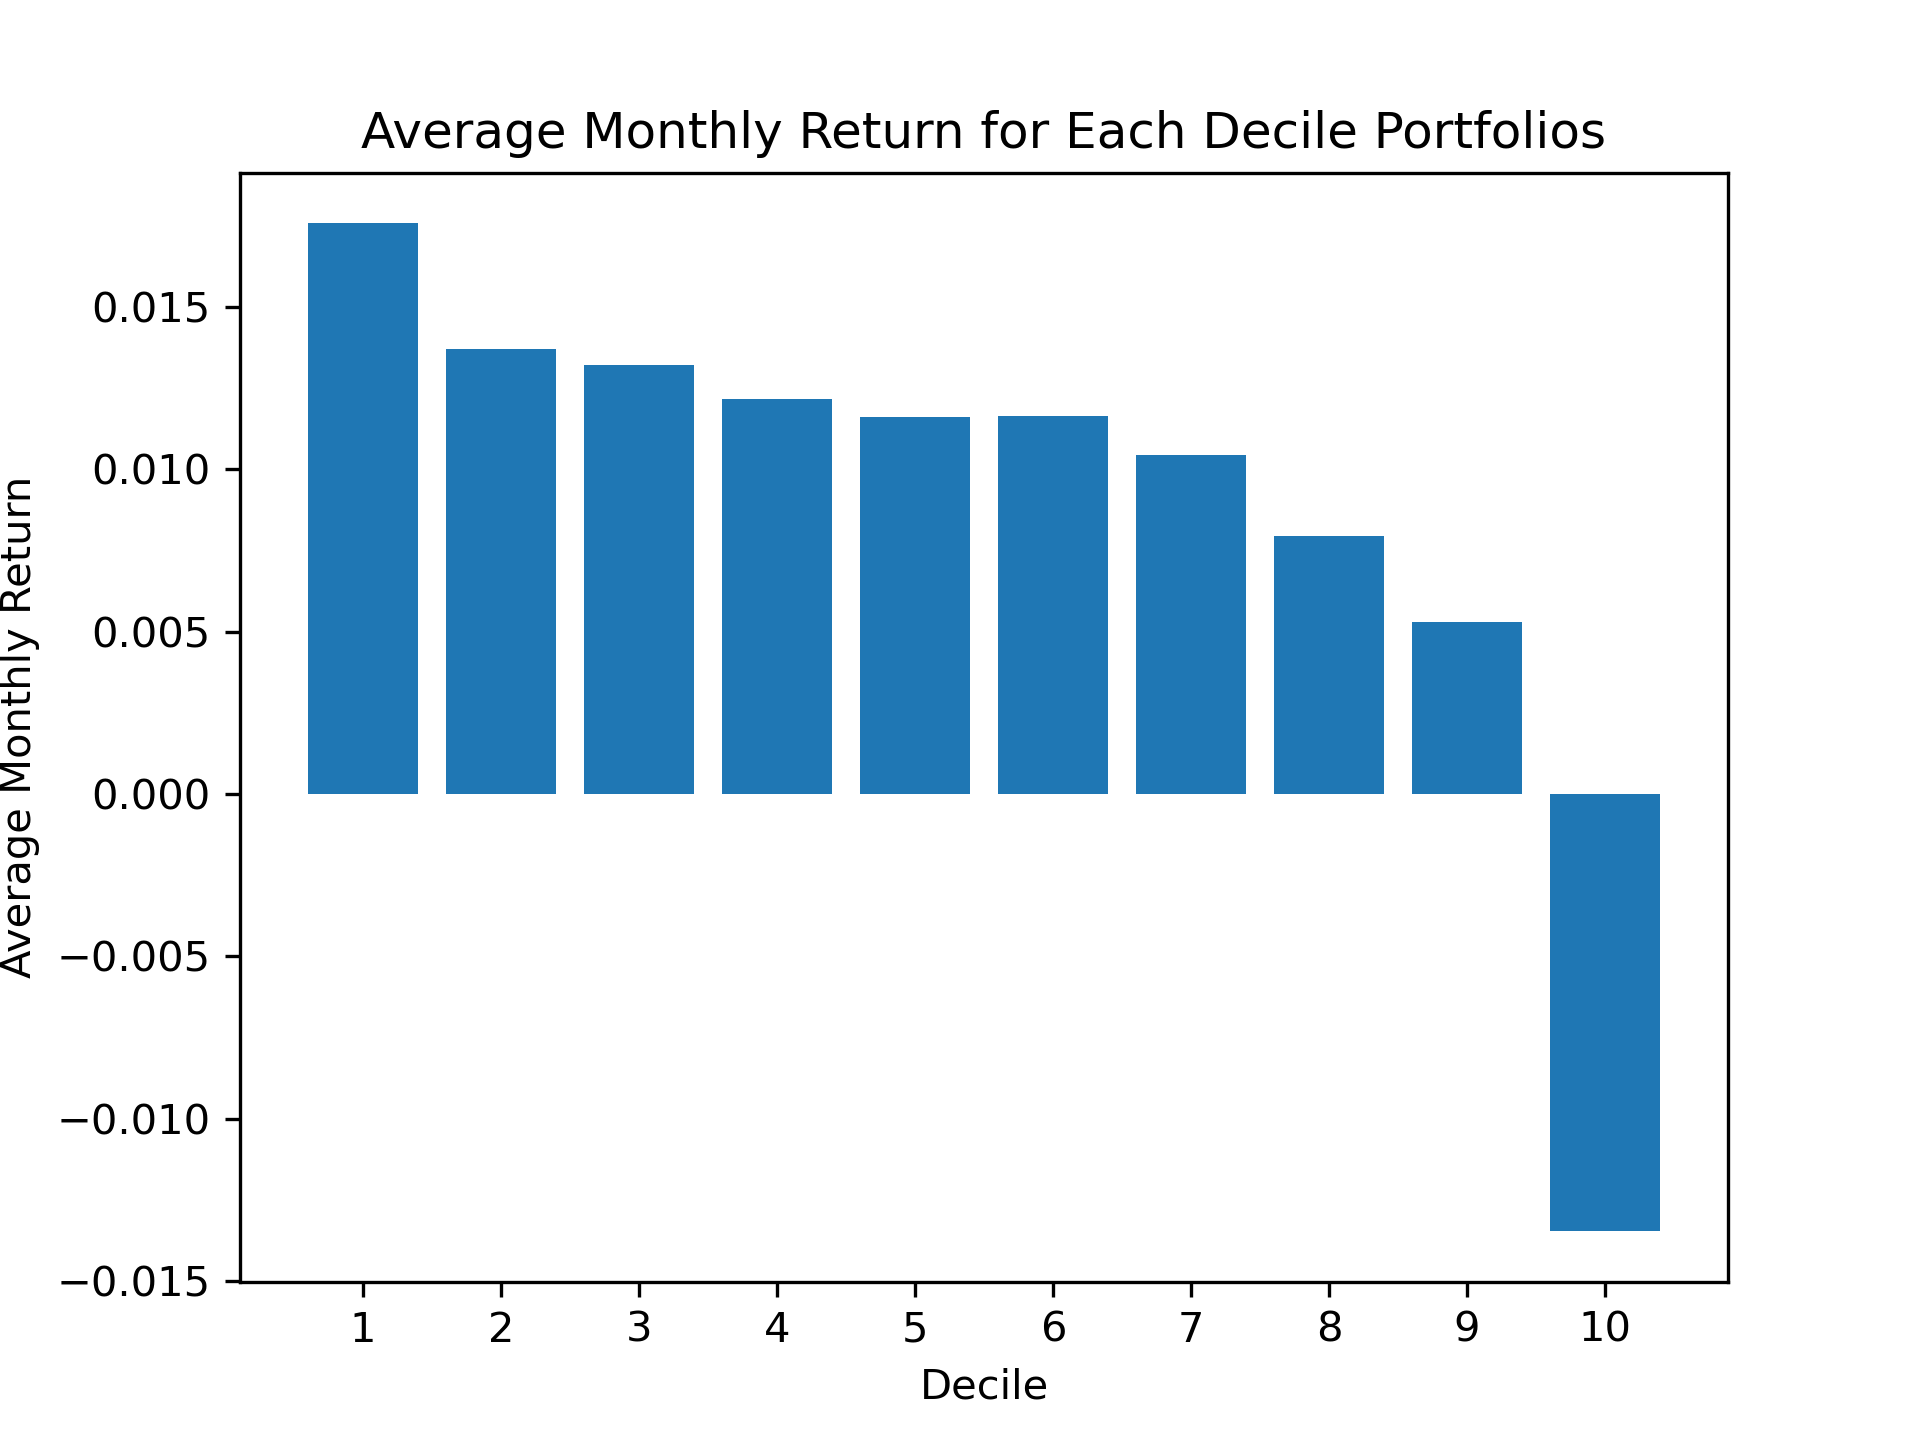
\includegraphics[width=0.85\textwidth]{data/q2_graph.png}
\caption{Average Monthly Return for Each Decile Portfolios}
\label{fig:example}
\end{figure}


\vspace{6mm}
\centering{\textbf{-- END --}}
